\section{Problem 1}

The exercise at the beginning asks for the best degree using some empirical risk. So for having some empirical results we will run the polyreg function in a variety of degrees. In general we use the degrees from 1 to 50. We choose this as the final plot it resembles the one in the example Function polyreg does exactly this when 3 arguments are given. We choose this as the final plot it resembles the one in the example.

The code for this problem is the \texttt{polyeg.m} and \texttt{hm1\_1.m}. The result for the empirical is that the lowest error comes with a 11th degree polynomial.

If we print all the empirical risks that we computed, we will see
that the lowest error is with the polynomial degrees 8,9,10,11
and the ones with degrees 12,13,14,15,16 are really close.
The errors are 0.0113 and 0.0114 respectively. So these degrees are reasonable.
\begin{figure}[!h]
{
    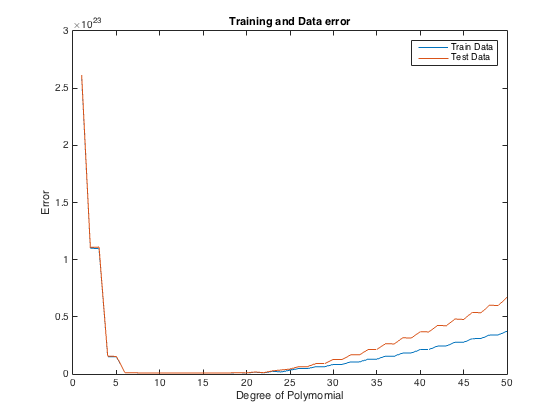
\includegraphics[width=\columnwidth]
    {figures/new.png}
    \caption{\footnotesize{\bf}Training and Testing loss}
    \label{fig:fold}
}
\end{figure}

In order to do 2-fold cross validation we split our data into 2 sets.
I use the randperm function to create an array with the numbers from
1 to 500. This will split the data in 2 random sets. Then we will 
run the polyreg function 2 times one with the 1st set as training and
the 2nd as testing and vice versa. Then we will average the 2 errors
between these 2 runs to give us the best degree of polynomial. From
our empirical measurement I believe that it should be between 8th and
15th degree (the plot is in figure \ref{fig:fold}).

The result of this procedure varies. This is because the training and
testing data differ in each run. But still at my runs, it is never lower than 8 or more than 15. This coincides with the empirical risk
we already found ( the plot for best dimension is figure \ref{fig:best_d}).

\begin{figure}[!h]
{
    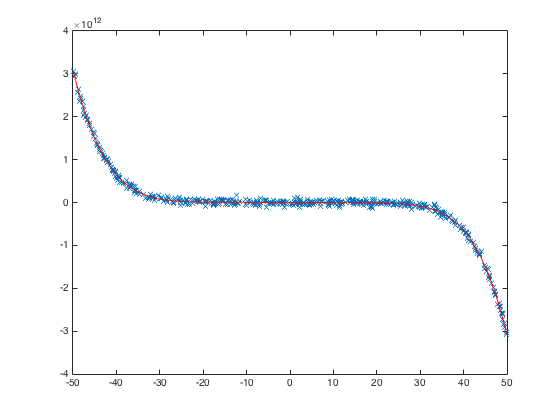
\includegraphics[width=\columnwidth]
    {figures/new2.png}
    \caption{\footnotesize{\bf} Data with the best polynomial from 2 fold.}
    \label{fig:best_d}
}
\end{figure}
\vspace{2 mm}
